\documentclass[10pt]{article}

\usepackage[a4paper, left=2cm, right=2cm]{geometry} % A4 paper size and thin margins

\usepackage{xcolor} % Required for specifying custom colours
\definecolor{grey}{rgb}{0.9,0.9,0.9} % Colour of the box surrounding the title

\usepackage{graphicx}
\usepackage[colorlinks=true, allcolors=black]{hyperref}
\usepackage{amsmath}
\usepackage{indentfirst}
\setlength{\parindent}{2em}

\usepackage[utf8]{inputenc} % Required for inputting international characters
\usepackage[T1]{fontenc} % Output font encoding for international characters
\usepackage[sfdefault]{ClearSans} % Use the Clear Sans font (sans serif)
%\usepackage{XCharter} % Use the XCharter font (serif)
\usepackage{float}

\newcommand{\tabincell}[2]{\begin{tabular}{@{}#1@{}}#2\end{tabular}} 	

\begin{document}
%----------------------------------------------------------------------------------------
%	TITLE PAGE
%----------------------------------------------------------------------------------------

\begin{titlepage} % Suppresses displaying the page number on the title page and the subsequent page counts as page 1
	
	%------------------------------------------------
	%	Grey title box
	%------------------------------------------------
	
	\colorbox{grey}{
		\parbox[t]{1.1\textwidth}{ % Outer full width box
			\parbox[t]{1.02\textwidth}{ % Inner box for inner right text margin
				\raggedleft % Right align the text
				\fontsize{34pt}{40pt}\selectfont % Title font size, the first argument is the font size and the second is the line spacing, adjust depending on title length
				\vspace{0.7cm} % Space between the start of the title and the top of the grey box
				
				< Journey Assistant >\\
                Software Design Model\\
                Version 2.0\\
				
				\vspace{0.7cm} % Space between the end of the title and the bottom of the grey box
			}
		}
	}
	
	\vfill % Space between the title box and author information
	
	%------------------------------------------------
	%	Author name and information
	%------------------------------------------------
	
	\parbox[t]{1\textwidth}{ % Box to inset this section slightly
		\raggedleft % Right align the text
		\large % Increase the font size
		{\Large Group Member}\\[4pt] % Extra space after name
        Yiwen Song\\
        Zhihui Xie\\
        Weizhe Wang\\
        Huangfei Jiang\\
        Haoping Chen\\
		% Institution Name\\[4pt] % Extra space before URL
		% \texttt{LaTeXTemplates.com}\\
		
		\hfill\rule{0.2\linewidth}{1pt}% Horizontal line, first argument width, second thickness
    }
    
	
\end{titlepage}

\newpage

\begin{center}
    {\LARGE Modification History}
    
    \begin{tabular}{|c|c|c|c|} 
        \hline 
        Date&Version&Description&Author\\
        \hline  
        2019-04-16&1.0&The first version of this document.&Huangfei Jiang \& Haoping Chen\\
		\hline 
        2019-06-18&2.0&Modify some description.&Zhihui Xie\\
		\hline
		& & & \\
		\hline
		& & & \\
		\hline
    \end{tabular}    
\end{center}

\newpage

\tableofcontents
\newpage

\section{Introduction}
\subsection{Purpose}
The purpose of this software design model is to collect and draw various models of our 'Journey Assistant' software. We will present the system structure in detail on the basis of former requirement specifications and system analysis, and lay the foundation of subsequent software implementation. This document will focus on our system and use UML to construct the Logic View, Implementation View, Process View, Deployment View, etc. It is designed for the development team to specify the various design models of the ‘Journey Assistant’ software, and base on which to start developing of this system.

\subsection{Scope}
This document is applied to our Journey Assistant System and other subsystems or models related with our software. It is a specialized document for our product.

\subsection{Definition}
There is no extra abbreviation shown in this document. Refer to our 'Glossary' document if any question occurs.

\subsection{Bibliography}
\begin{itemize}
  \item[(1)] <Feasibility Study Feedback> (GB8567-88)
  \item[(2)] <Object Oriented Software Engineering (Version 3)> (Tsinghua University Press)
  \item[(3)] <Object Oriented Software Engineering Practice Guidelines>
\end{itemize}

\subsection{Summary}
This document includes models of the following 5 parts: 'Use Case View', 'Logic View', 'Implementation View', 'Process View' and 'Deployment View'. 'Use Case View' presents all possible use cases of the system. 'Logic View' mainly includes system architecture diagram, design class diagram and implementation of the use case. 'Implementation View' construct component diagrams for each subsystem. 'Process View' uses class diagrams and component diagrams to represent the processes and threads of the system. 'Deployment View' presents software and hardware implementation of the system. Each part of this document is closely related with each other, and present the design model of the system jointly.

\section{Use Case View}

\begin{figure}[H]
    \centering
    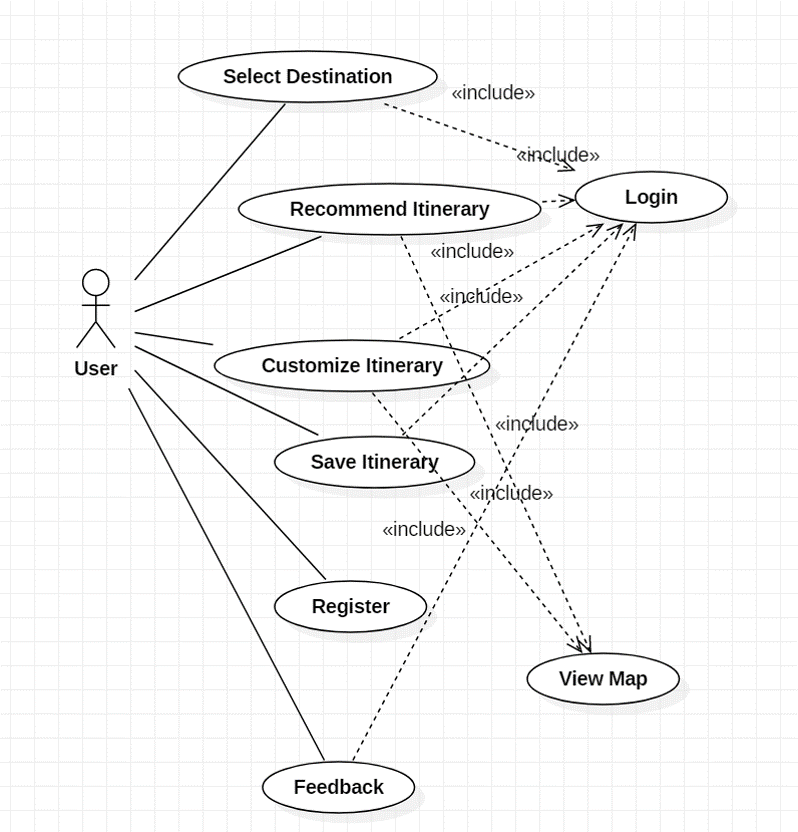
\includegraphics[width=14cm]{usecase.png}
    \caption{Use Case View}
    \label{Use Case View}
\end{figure}

\section{Logic View}
\subsection{System Architecture}
The whole system can be decomposed into 4 subsystems: UI subsystem, user management subsystem, journey management subsystem, and reedback management subsystem.

\begin{figure}[H]
    \centering
    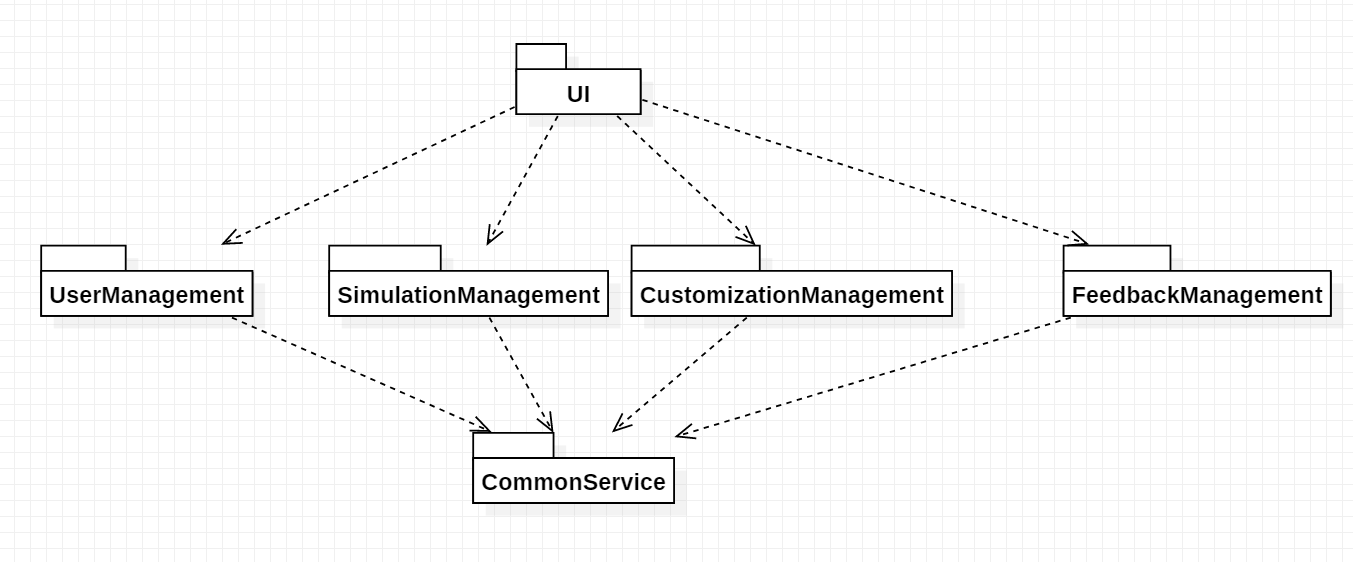
\includegraphics[width=14cm]{architecture.png}
    \caption{System Architecture}
    \label{System Architecture}
\end{figure}

The following class diagrams (Figure \ref{UI Subsystem} - \ref{Feedback Management Subsystem}) show inner logic for every package.

\begin{figure}[H]
    \centering
    
    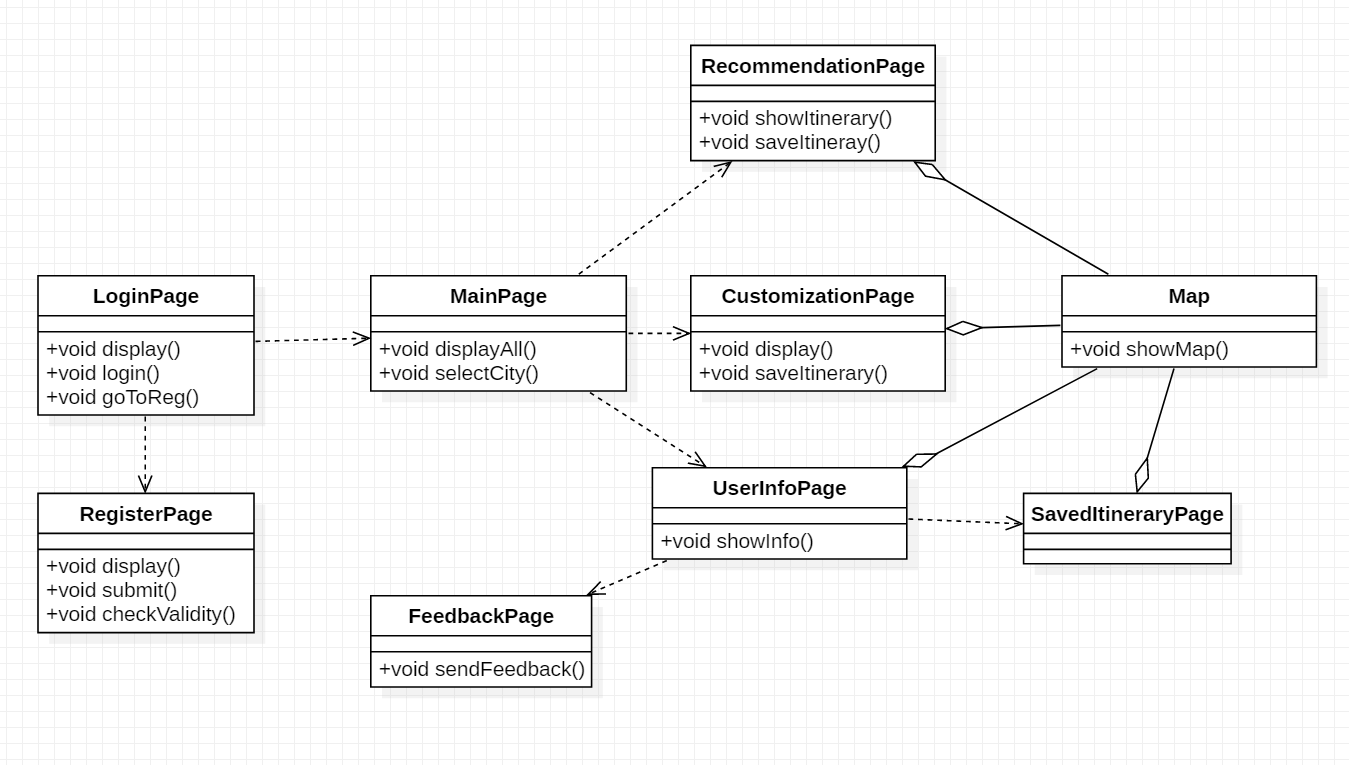
\includegraphics[width=14cm]{ui.png}
    \caption{UI Subsystem}
    \label{UI Subsystem}
\end{figure}

\begin{figure}[H]
    \centering
    
    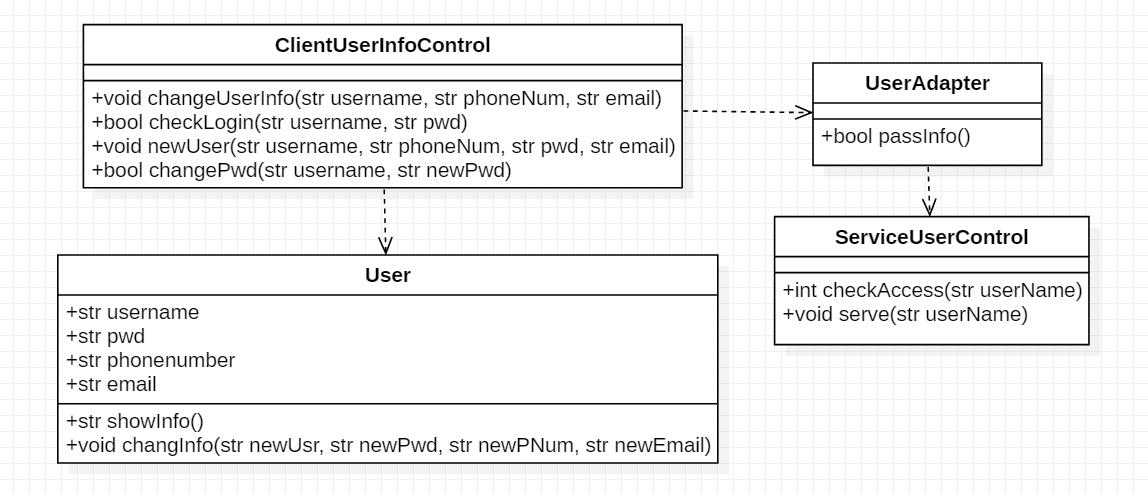
\includegraphics[width=14cm]{usermanager.jpg}
    \caption{User Management Subsystem}
    \label{User Management Subsystem}
\end{figure}

\begin{figure}[H]
    \centering
    
    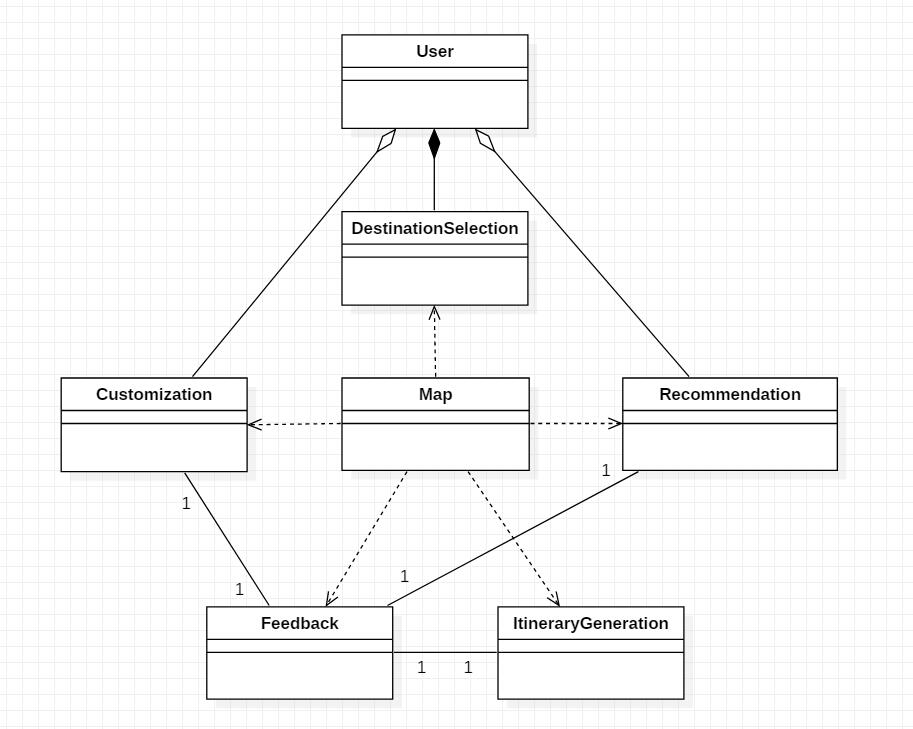
\includegraphics[width=14cm]{journeymanager.jpg}
    \caption{Journey Management Subsystem}
    \label{Journey Management Subsystem}
\end{figure}

\begin{figure}[H]
    \centering
    
    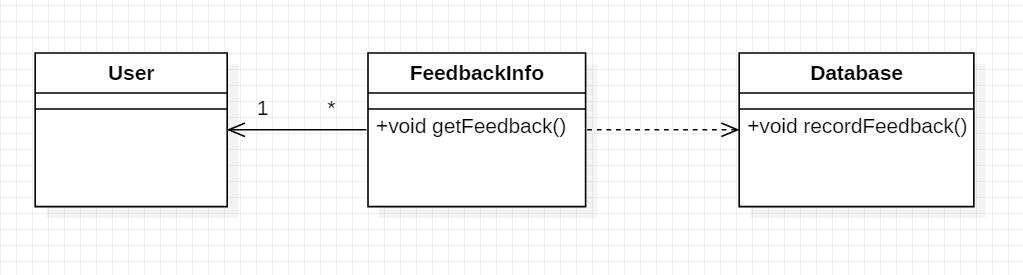
\includegraphics[width=14cm]{reportmanager.jpg}
    \caption{Feedback Management Subsystem}
    \label{Feedback Management Subsystem}
\end{figure}

\subsection{Use Case Realization}
For each type of use case, we use an interaction diagram to display our corresponding inner design.

\subsubsection{Log-in Realization}
\begin{figure}[H]
    \centering
    
    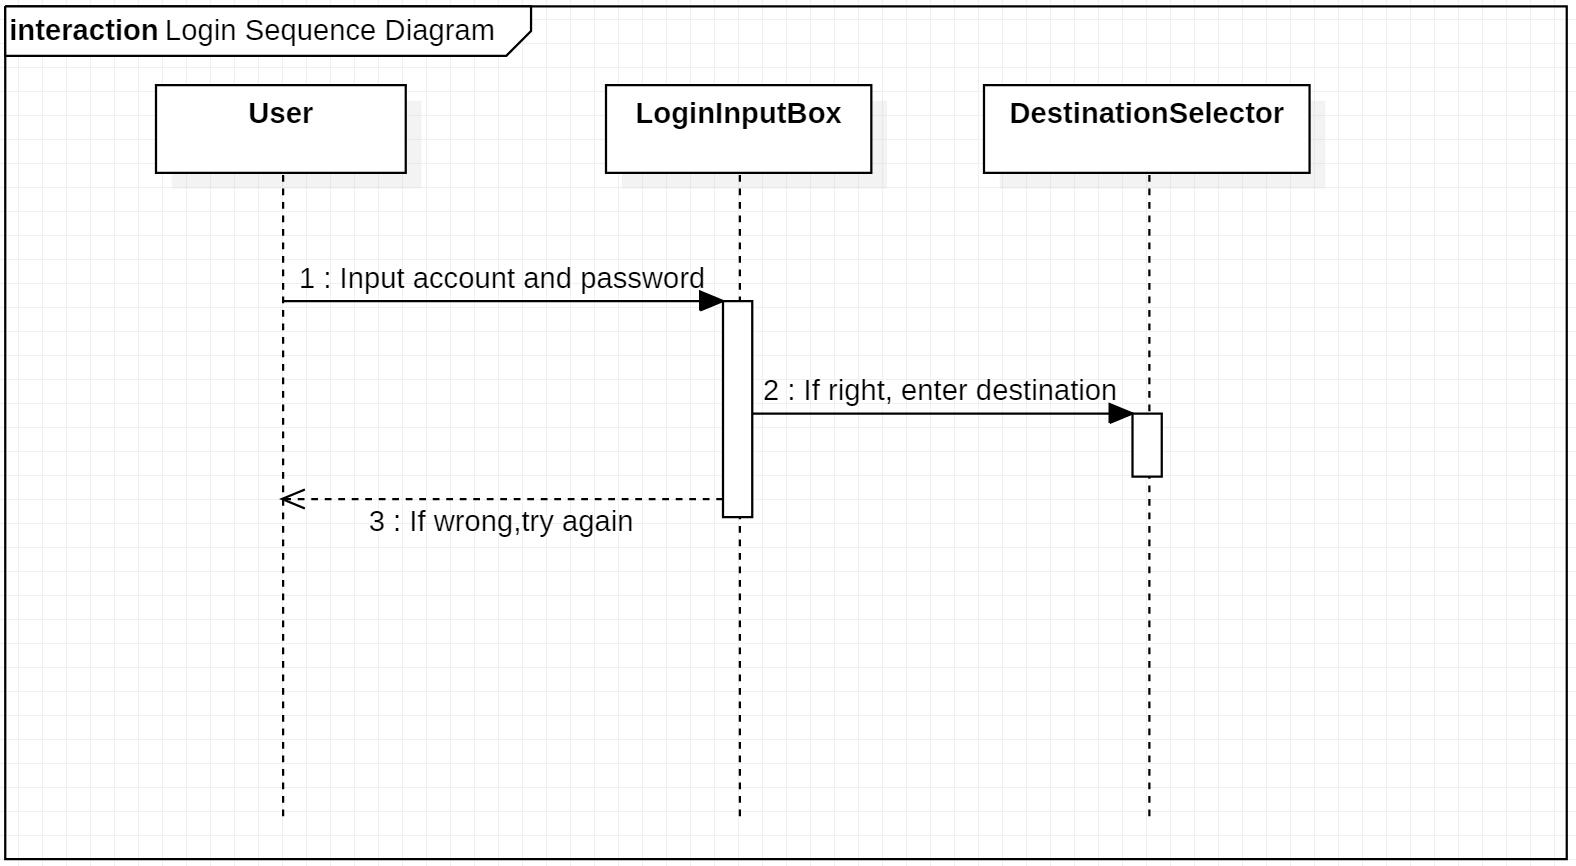
\includegraphics[width=14cm]{login.jpg}
    \caption{Log-in Sequence Diagram}
    \label{Log-in Sequence Diagram}
\end{figure}

\subsubsection{Recommendation Realization}

\begin{figure}[H]
    \centering
    
    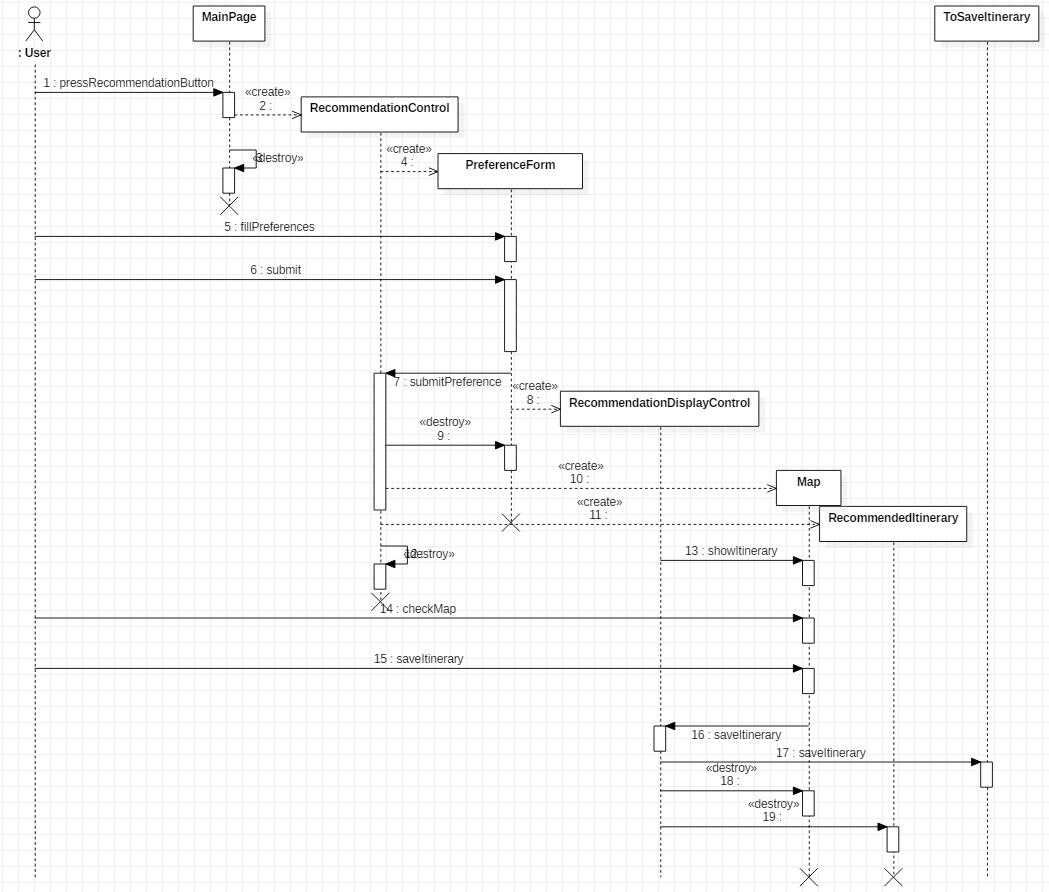
\includegraphics[width=14cm]{recommendation.png}
    \caption{Recommendation Sequence Diagram}
    \label{Recommendation Sequence Diagram}
\end{figure}

\subsubsection{Feedback Realization}
\begin{figure}[H]
    \centering
    
    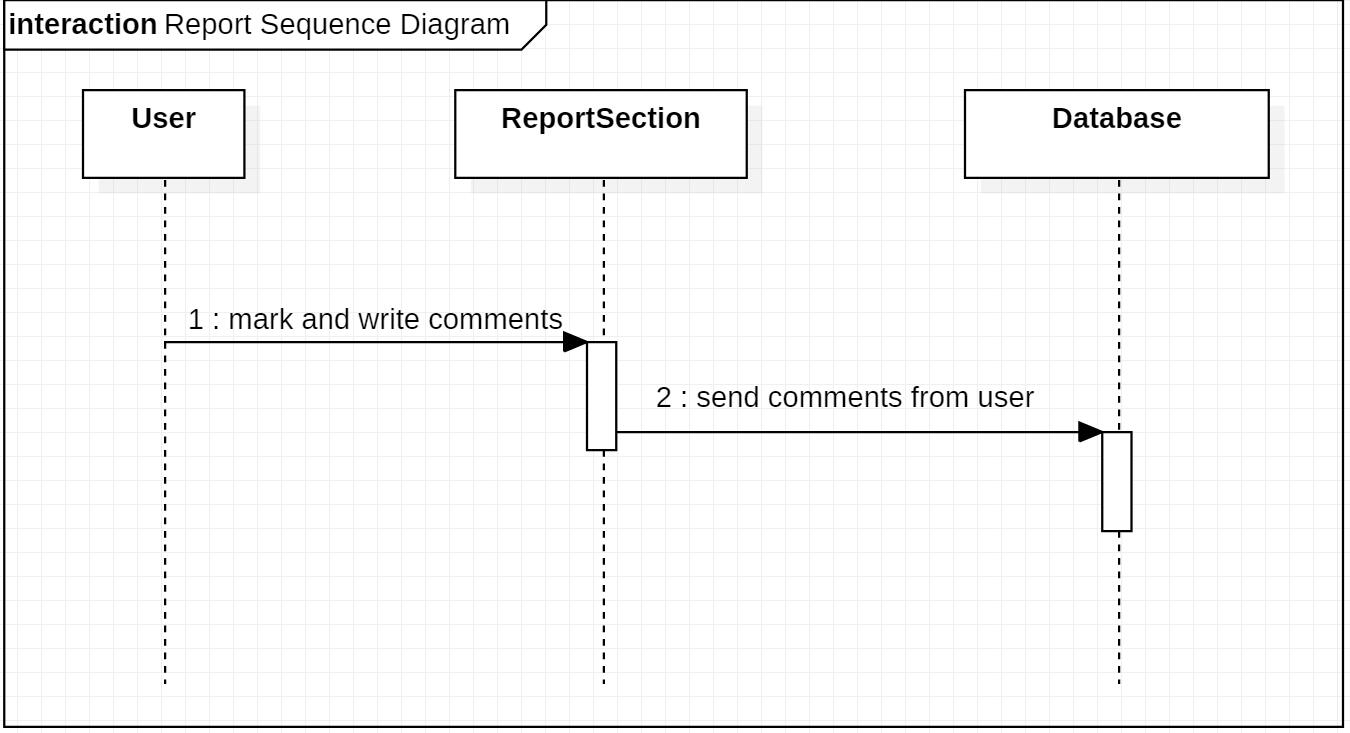
\includegraphics[width=14cm]{report.jpg}
    \caption{Feedback Sequence Diagram}
    \label{Feedback Sequence Diagram}
\end{figure}

\subsection{Design Class Diagram}
We list all the class diagrams for every corresponding package in Figure \ref{UI Subsystem} -\ref{CommonService Subsystem}.

\begin{figure}[H]
    \centering
    
    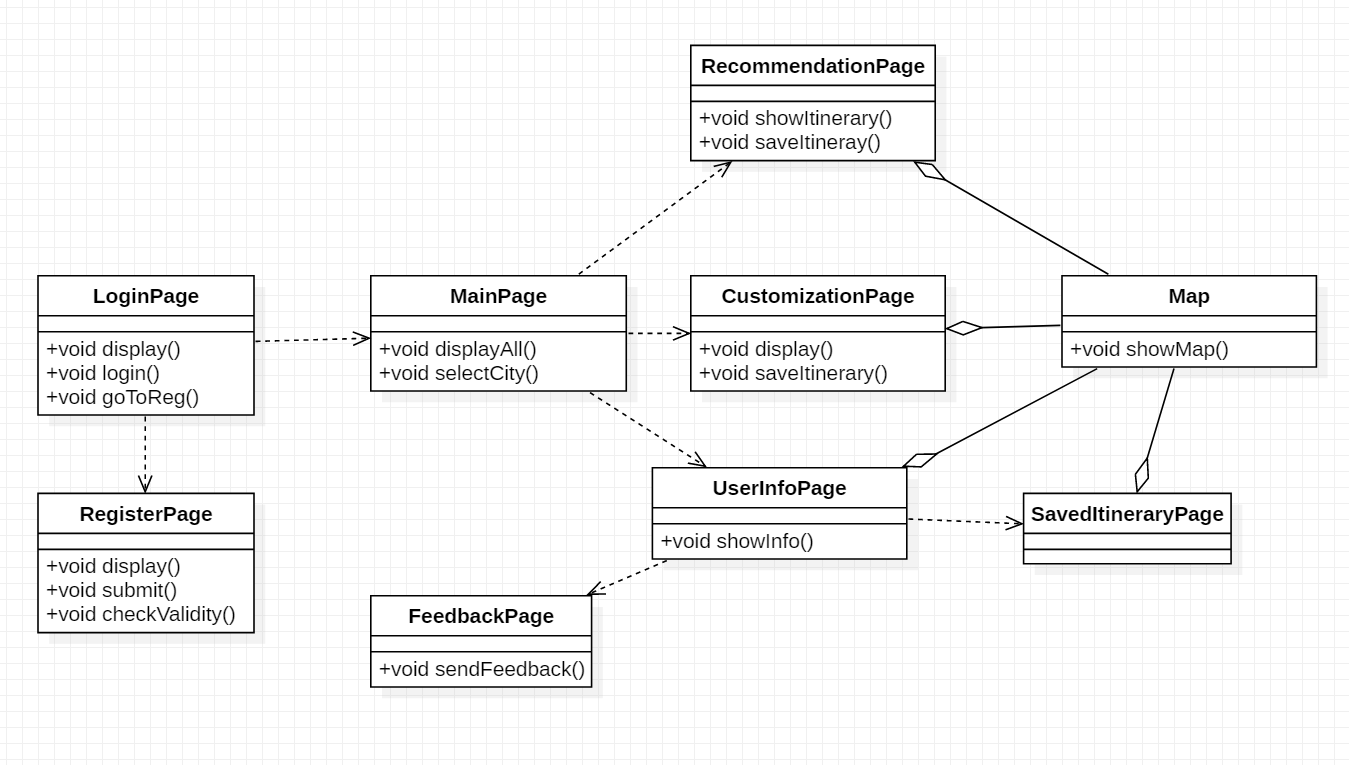
\includegraphics[width=14cm]{ui.png}
    \caption{UI Subsystem}
    \label{UI Subsystem}
\end{figure}

\begin{figure}[H]
    \centering
    
    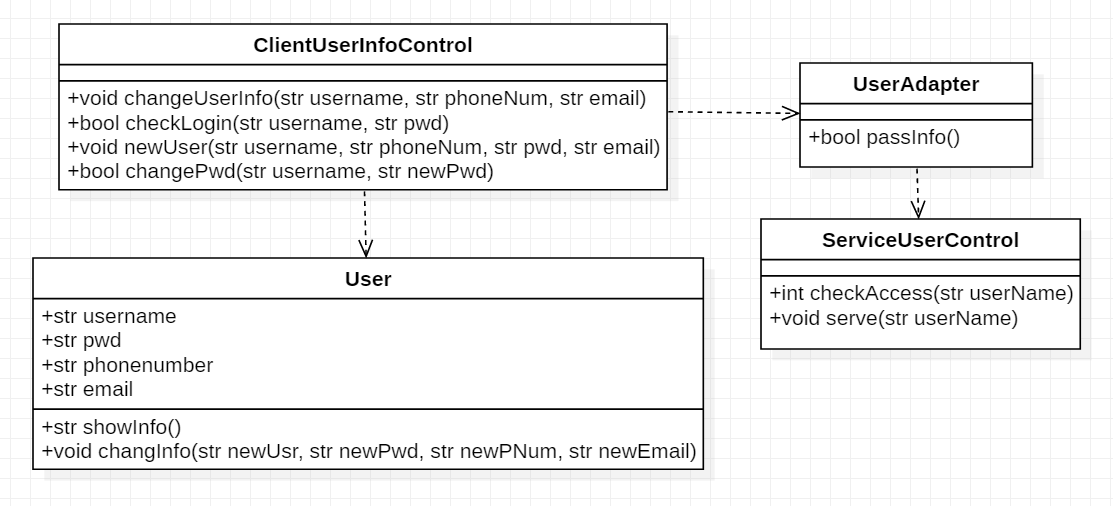
\includegraphics[width=14cm]{usermanagement.png}
    \caption{UserManagement Subsystem}
    \label{UserManagement Subsystem}
\end{figure}

\begin{figure}[H]
    \centering
    
    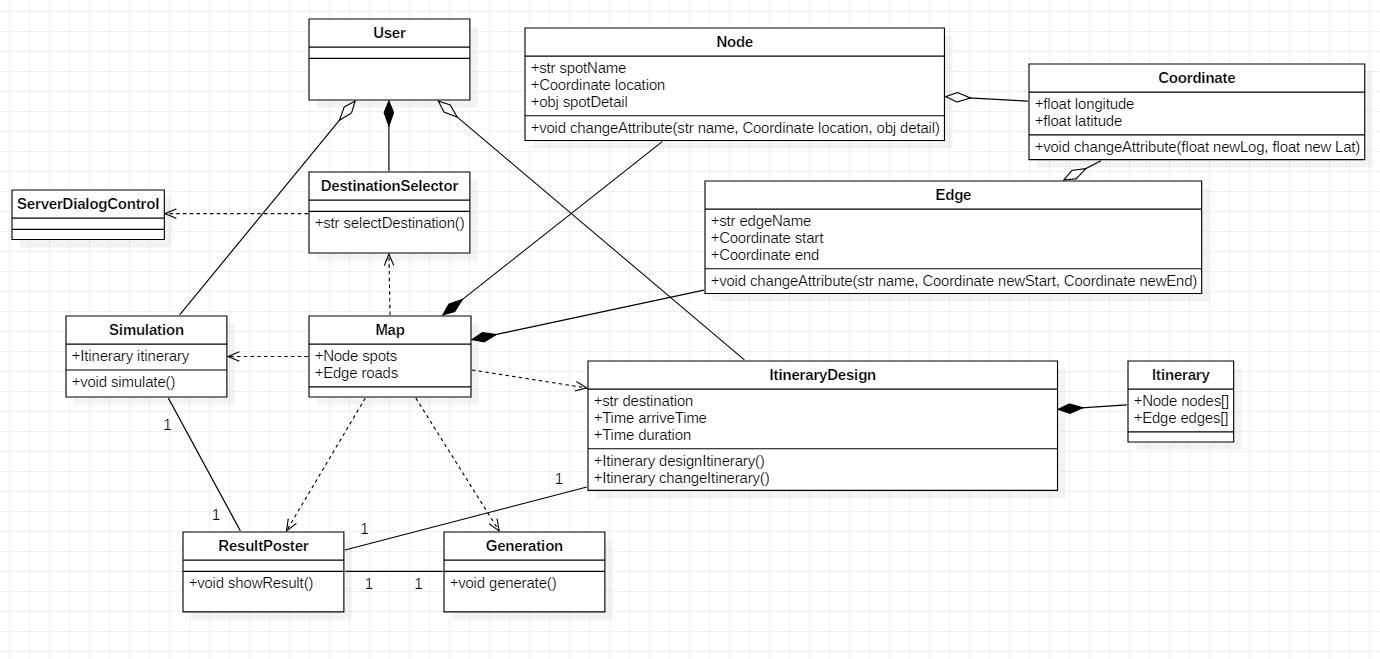
\includegraphics[width=14cm]{journeymanagement.png}
    \caption{JourneyManagement Subsystem}
    \label{JourneyManagement Subsystem}
\end{figure}

\begin{figure}[H]
    \centering
    
    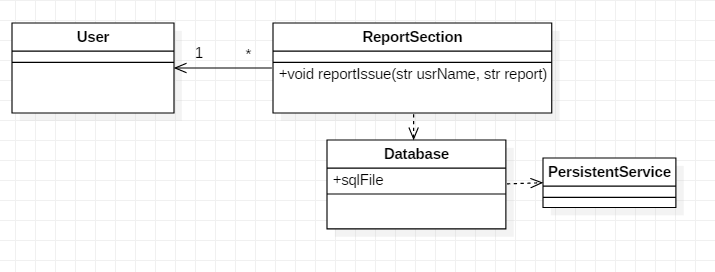
\includegraphics[width=14cm]{reportmanagement.png}
    \caption{FeedbackManagement Subsystem}
    \label{FeedbackManagement Subsystem}
\end{figure}

\begin{figure}[H]
    \centering
    
    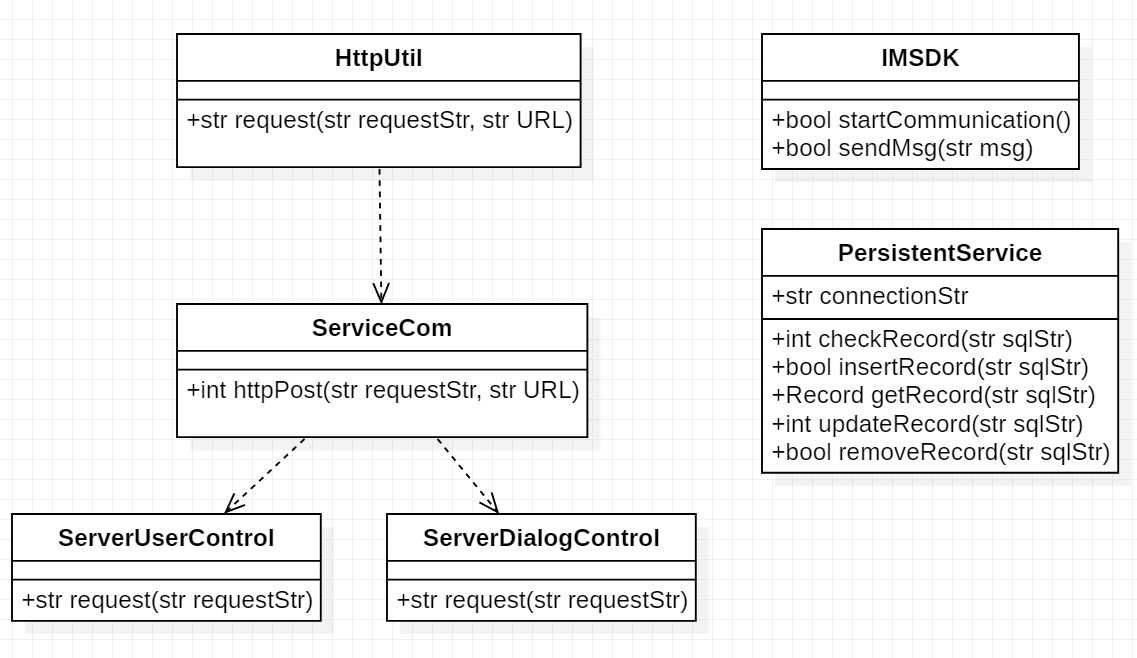
\includegraphics[width=14cm]{commonmanagement.png}
    \caption{CommonService Subsystem}
    \label{CommonService Subsystem}
\end{figure}

\subsection{Other Diagram}
None.

\section{Implementation View}

\subsection{Organization of our Development Model}
\subsubsection{User Management Subsystem}

\begin{figure}[H]
    \centering
    
    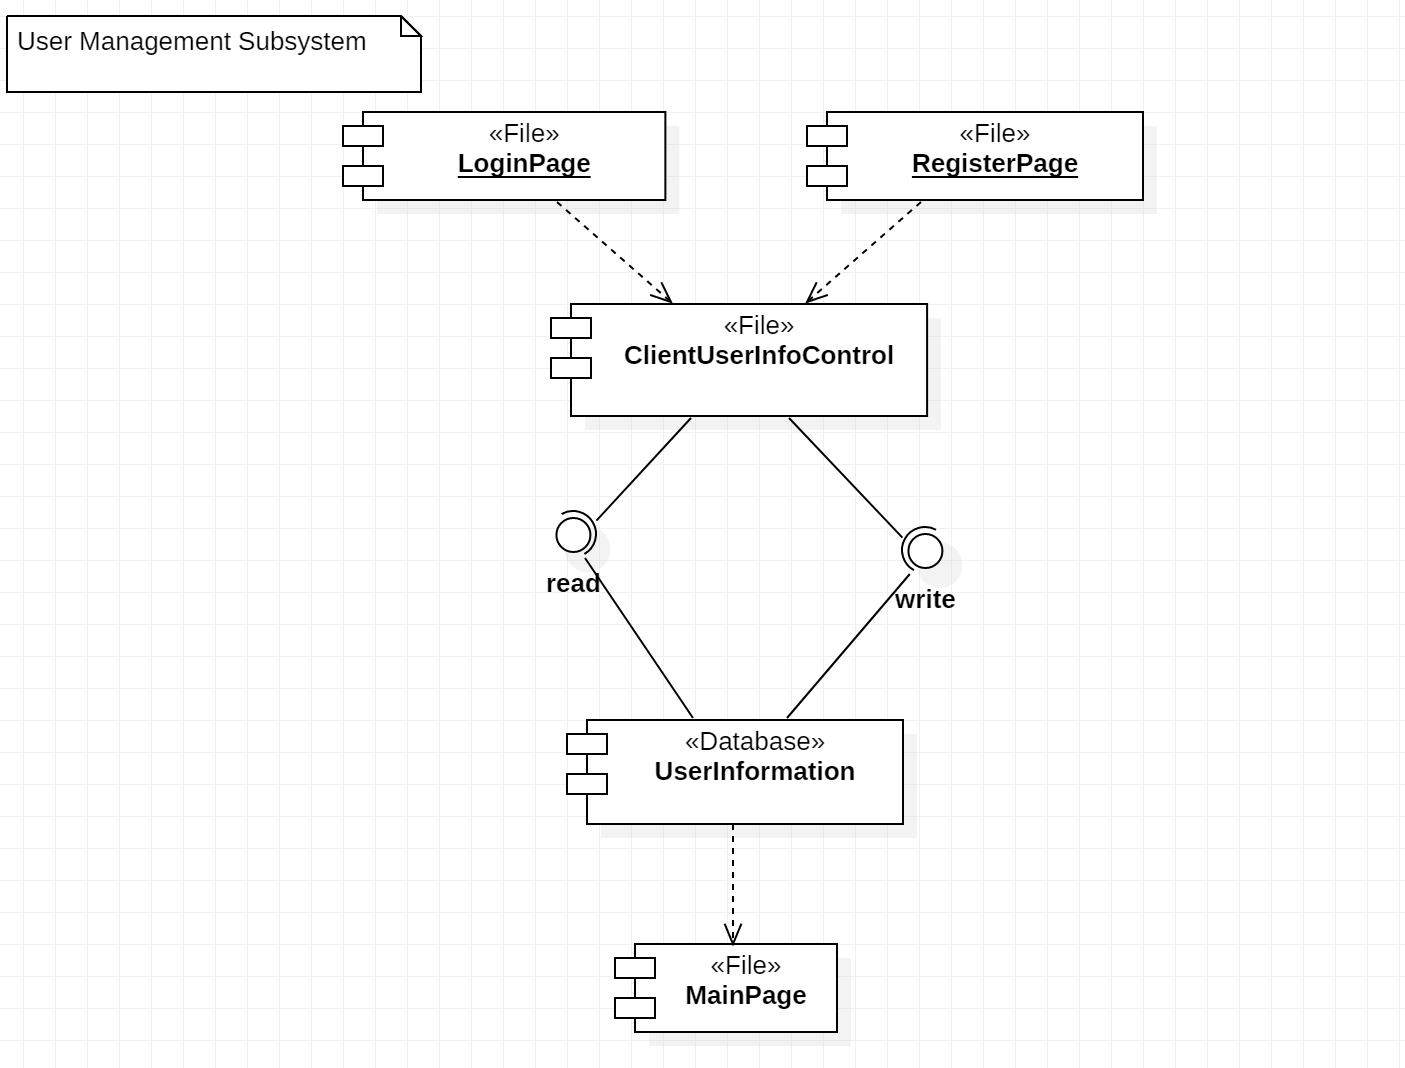
\includegraphics[width=14cm]{userbefore.png}
    \caption{User Management Subsystem}
    \label{User Management Subsystem}
\end{figure}

\subsubsection{Journey Management Subsystem}
\begin{figure}[H]
    \centering
    
    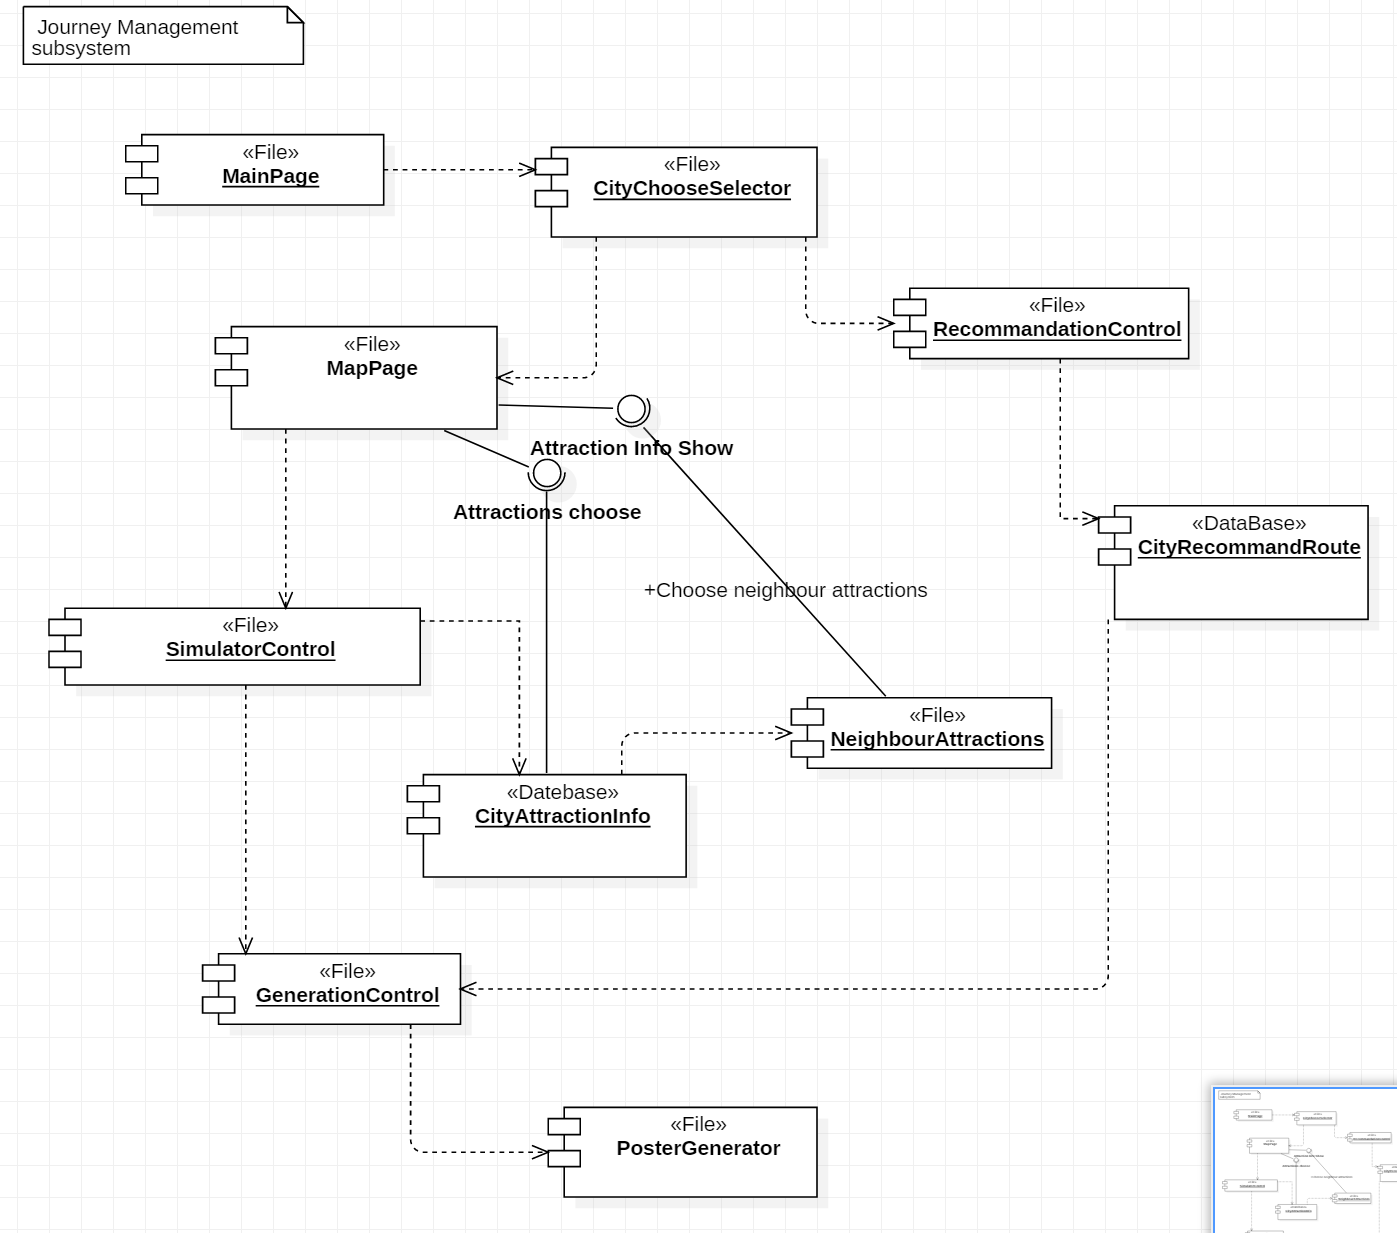
\includegraphics[width=14cm]{journeybefore.png}
    \caption{Journey Management Subsystem}
    \label{Journey Management Subsystem}
\end{figure}

\subsubsection{Feedback Subsystem}
\begin{figure}[H]
    \centering
    
    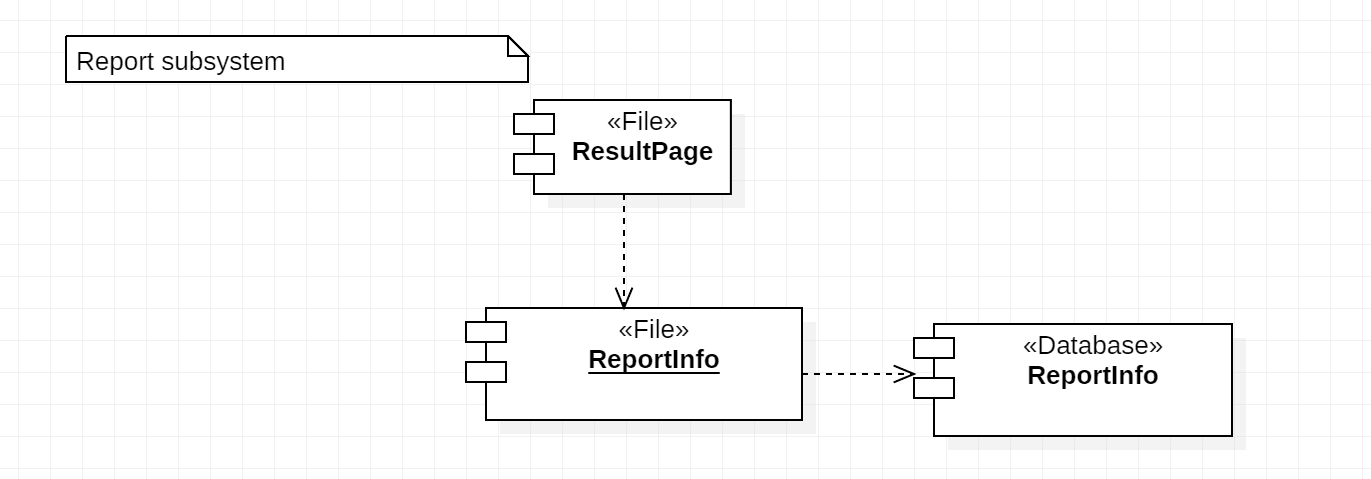
\includegraphics[width=14cm]{reportbefore.png}
    \caption{Feedback Subsystem}
    \label{Feedback Subsystem}
\end{figure}

\subsubsection{Commmon Service Subsystem}
\begin{figure}[H]
    \centering
    
    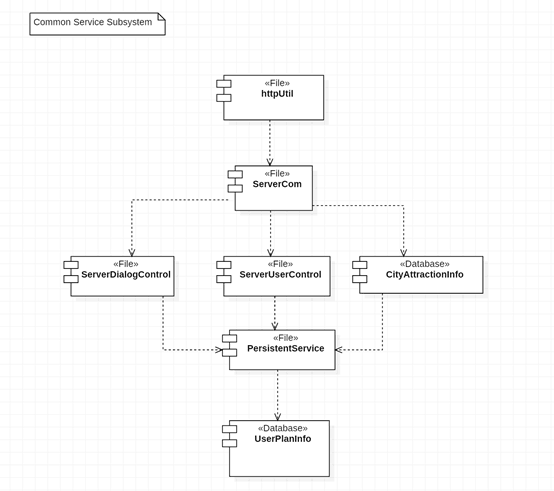
\includegraphics[width=14cm]{commonbefore.png}
    \caption{Commmon Management Subsystem}
    \label{Commmon Management Subsystem}
\end{figure}

\subsection{After Compiling}
\subsubsection{User Management Subsystem}

\begin{figure}[H]
    \centering
    
    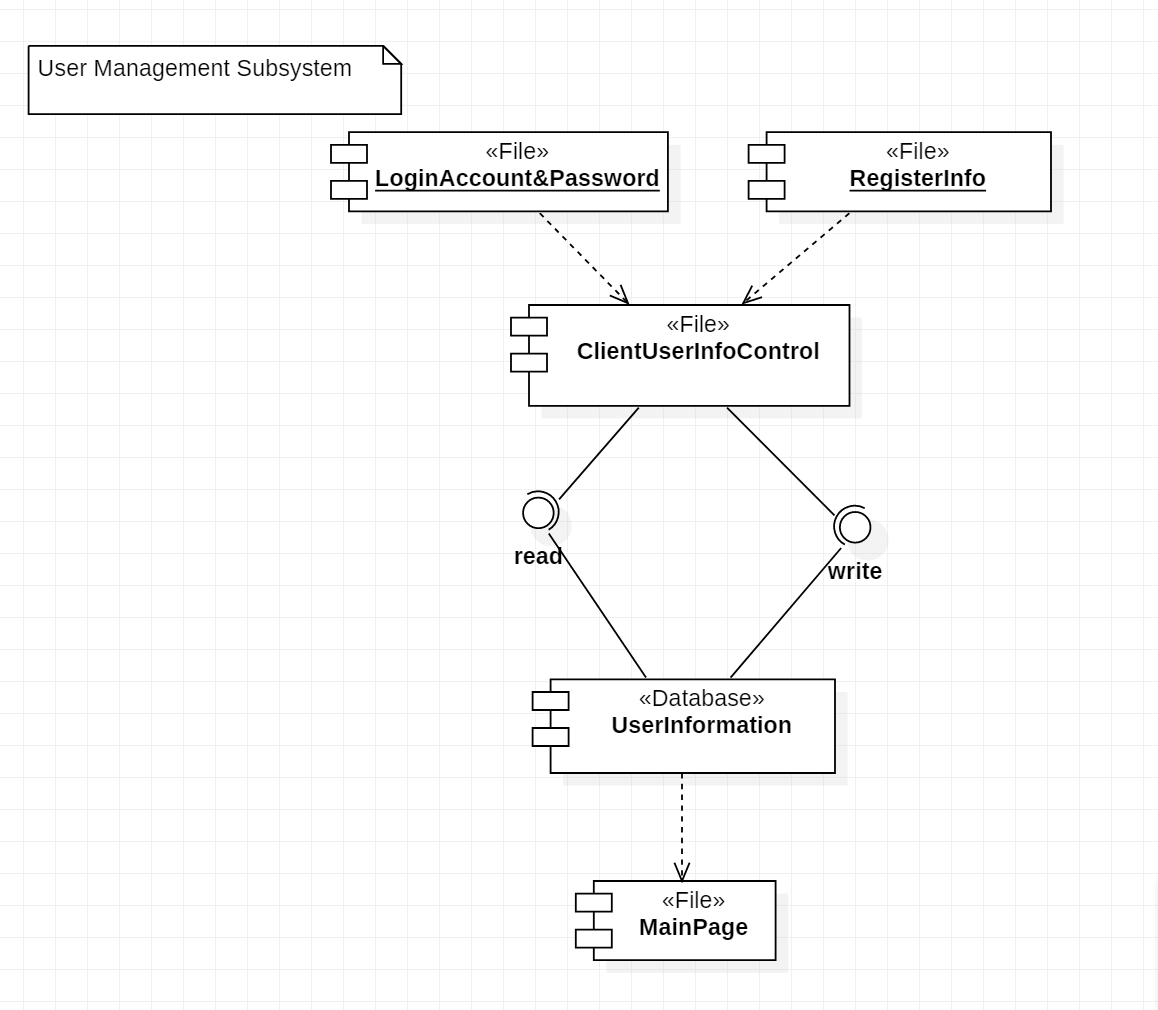
\includegraphics[width=14cm]{userafter.png}
    \caption{User Management Subsystem}
    \label{User Management Subsystem 2}
\end{figure}

\subsubsection{Journey Management Subsystem}
\begin{figure}[H]
    \centering
    
    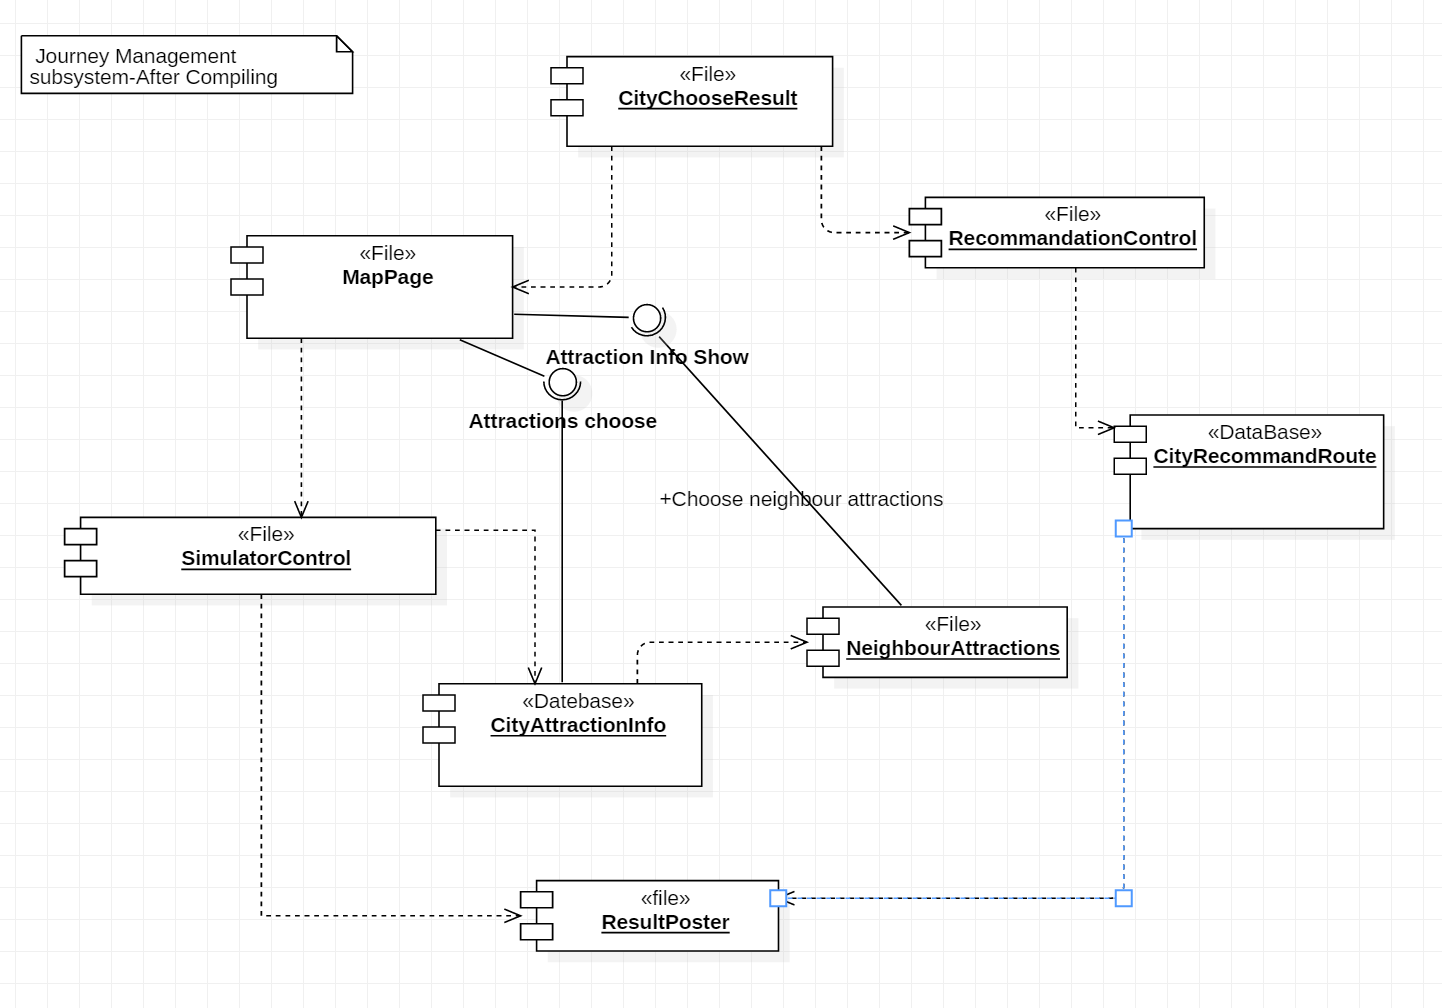
\includegraphics[width=14cm]{journeyafter.png}
    \caption{Journey Management Subsystem}
    \label{Journey Management Subsystem 2}
\end{figure}

\subsubsection{Feedback Subsystem}
\begin{figure}[H]
    \centering
    
    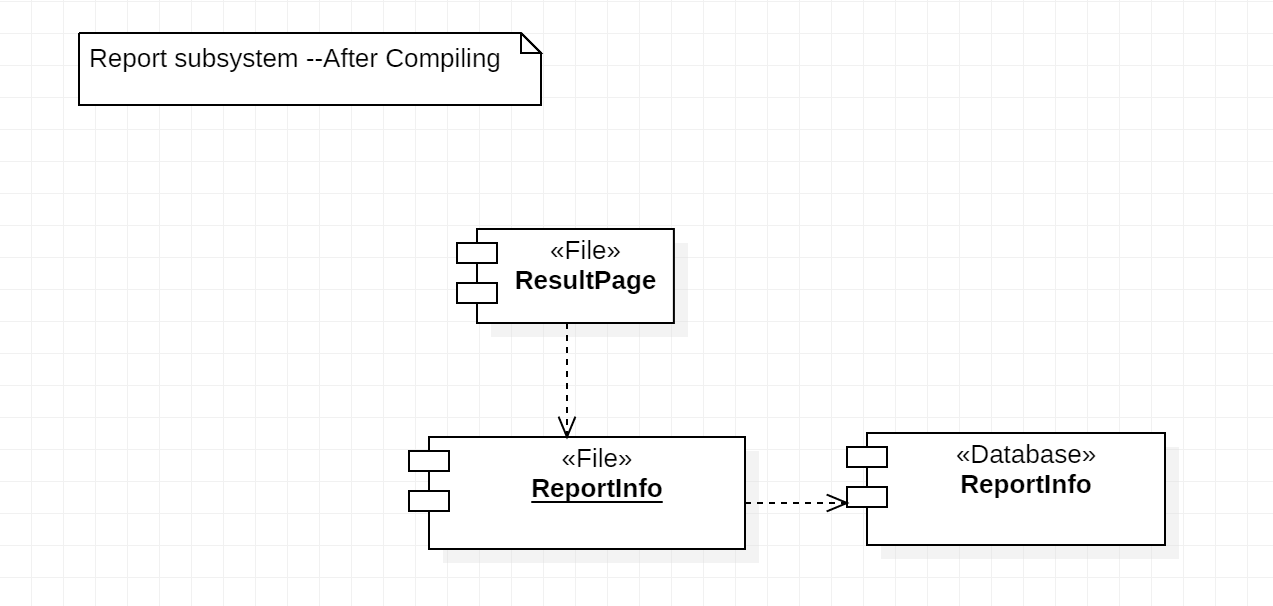
\includegraphics[width=14cm]{reportafter.png}
    \caption{Feedback Subsystem}
    \label{Feedback Subsystem 2}
\end{figure}

\subsubsection{Commmon Service Subsystem}
\begin{figure}[H]
    \centering
    
    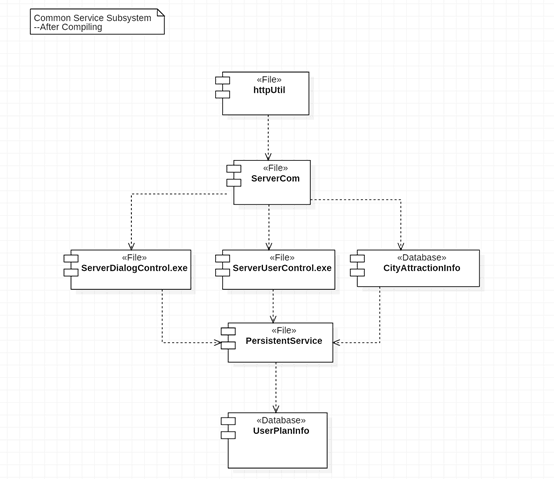
\includegraphics[width=14cm]{commonafter.png}
    \caption{Commmon Management Subsystem}
    \label{Commmon Management Subsystem 2}
\end{figure}

\section{Process View}
We use class diagram to present process class, thread class, and their interrelation.

\subsection{Client Process Diagram}
To improve user experiment, UI thread is only in charge of interaction between the user and boundary objects. For every controller and communication module, we use one individual thread. In this case application would not be hindered by frontend and communication tasks.

\begin{figure}[H]
    \centering
    
    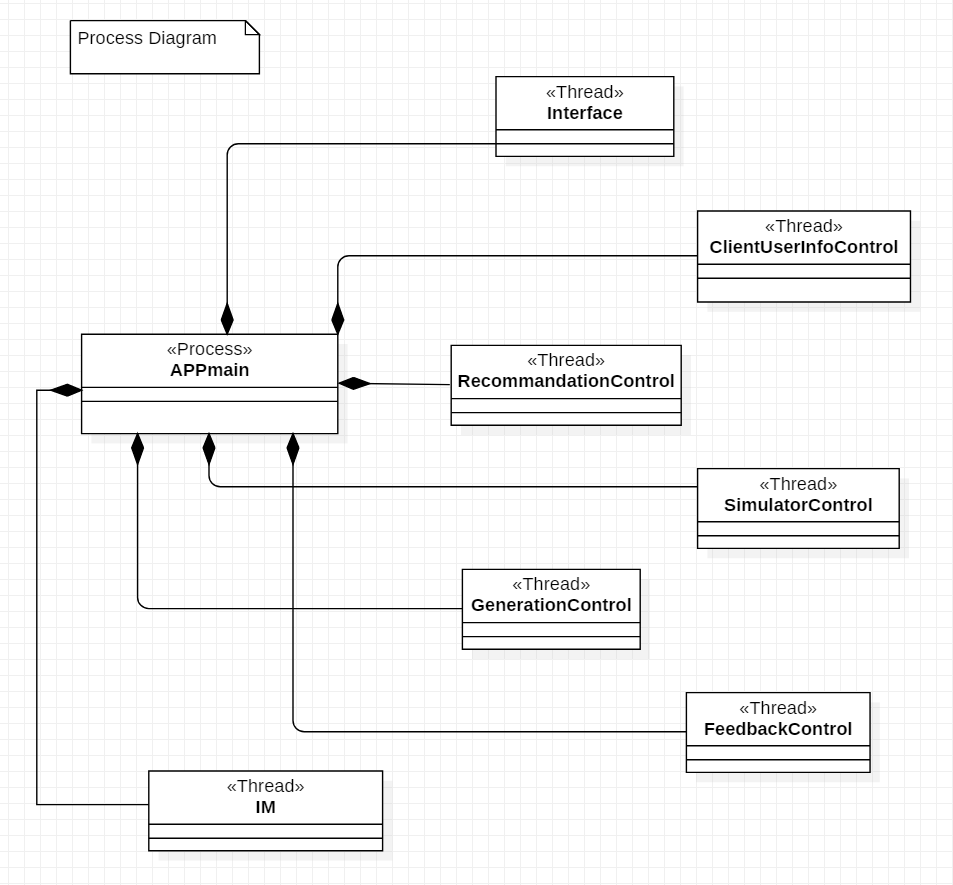
\includegraphics[width=14cm]{process.png}
    \caption{Client Process Diagram}
    \label{Client Process Diagram}
\end{figure}

\subsection{Server Process Diagram}
Because server process is very similar to client process, we omit it here.

\section{Deployment View}
Since our client app runs on mobile phone, we need the server play the backend role so that data access can be done directly via database server.

\begin{figure}[H]
    \centering
    
    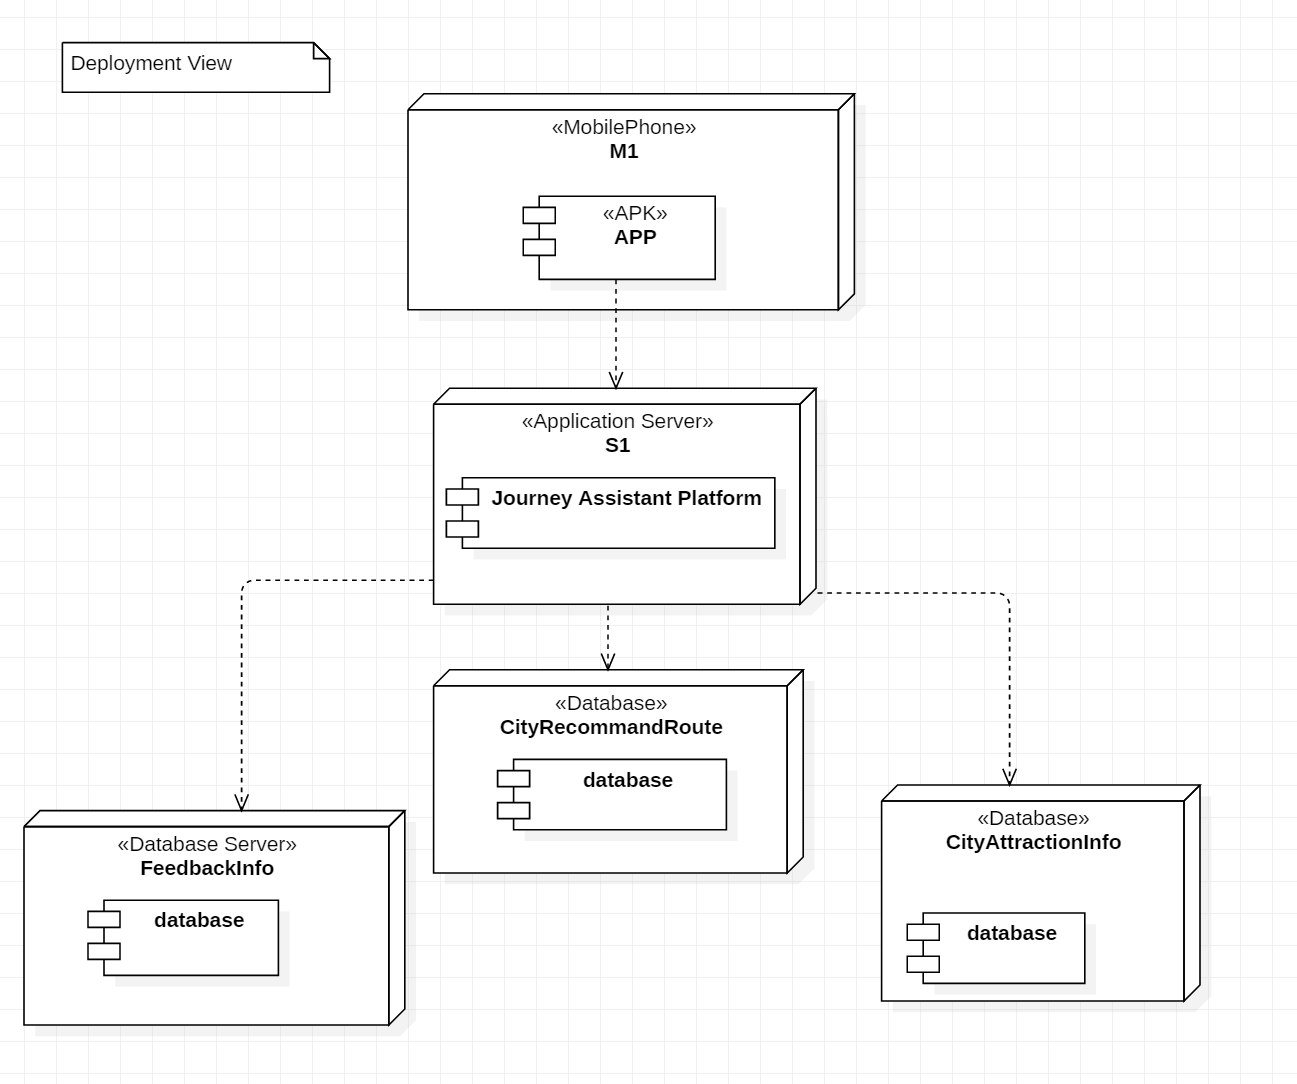
\includegraphics[width=14cm]{deploy.png}
    \caption{Deployment Diagram}
    \label{Deployment Diagram}
\end{figure}

\end{document}
